\documentclass[../main.tex]{subfiles}

\begin{document}
    Mit den optimierten Parametern kann der FID nun charakterisiert werden. Dazu wird ein FID mit den optimierten Parametern für die Wasserflasche aufgenommen. Dieser ist in Abb. \ref{fig:FID_Optimised} gezeigt.
    \begin{figure}[H]
        \centering
        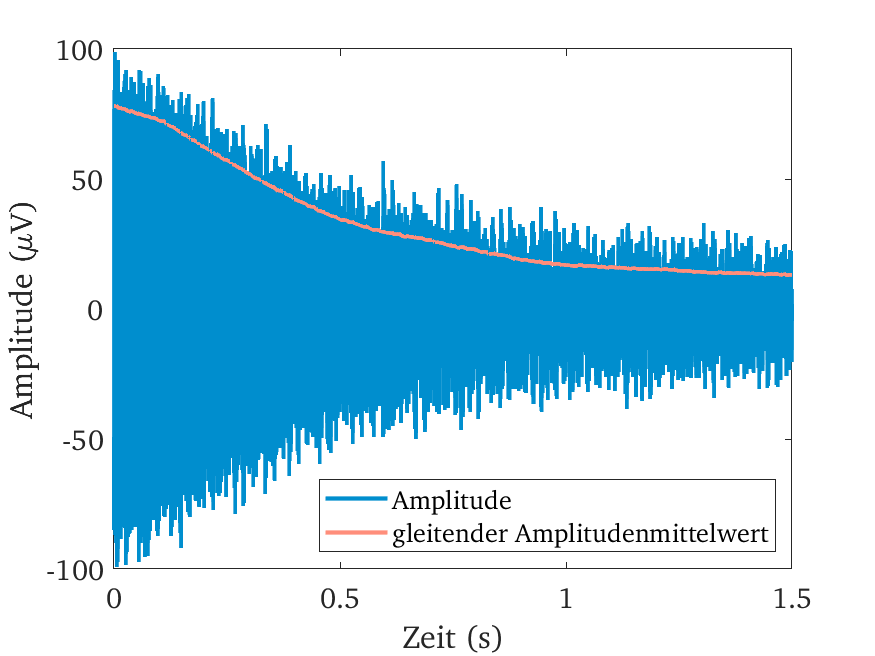
\includegraphics[width=\textwidth]{Bilddateien/7/Part7_Fig_1.png}
        \caption{FID einer Wasserflasche mit optimierten Parametern. Zur besseren Erkennbarkeit wurde eine Mittelung der Amplituden in den FID gelegt.}
        \label{fig:FID_Optimised}
    \end{figure}
    Aus der Messung ist gut zu erkennen, dass die Amplitude des FID mit der Zeit abnimmt und in das Rauschen übergeht. Zur Verdeutlichung ist ein gleitender Mittelwert der Amplitude in der Grafik mit aufgetragen. Nimmt man nun den höchsten Peak und bestimmt das Signal-Rausch-Verhältnis (SNR) erhält man einen Wert von \SI{4,8}{\deci \bel}. Aus dem FID lassen sich die gewünschten Zusammenhänge schwer ablesen. Da man an der Larmorfrequenz interessiert ist, wird im weiteren Verlauf die Fouriertransformation des FIDs betrachtet. Diese ist in Abb. \ref{fig:FID_Optimised} dargestellt.
    \begin{figure}[H]
        \centering
        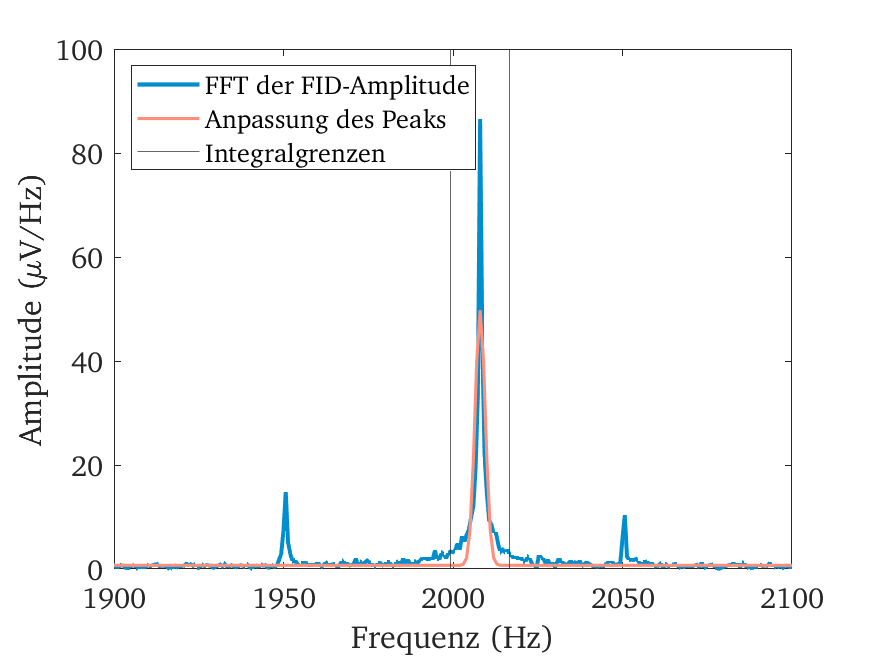
\includegraphics[width=\textwidth]{Bilddateien/7/Part7_Fig_2.png}
        \caption{Fouriertransformation des FID der Wasserflasche aus Abb. \ref{fig:FID_Optimised}.}
        \label{fig:FID_Optimised_FFT}
    \end{figure}
    Dabei wurde nur der Bereich von \SIrange{1900}{2100}{\hertz} abgebildet, um die Übersichtlichkeit zu bewahren. Die Peaks bei \SI{1950}{\hertz} und \SI{2050}{\hertz} sind auf die in der Netzspannung üblichen \SI{50}{\hertz} zurückzuführen. Bei \SI{2008}{\hertz} gibt es einen Peak. Dieser ist auf die Larmorpräzession in der Wasserprobe zurückzuführen. Die Breite des Peaks lässt sich Mittels einer Gaußfitfunktion bestimmen. Diese passt leider nicht ganz zum Peak. Es wurde die Fitfunktion gewählt, die am besten gepasst hat. Als breite wurde eine Standardunsicherheit $\sigma$ definiert. Diese beträgt $\sigma = \SI{1,5}{\hertz}$. Das Integral unter dem Peak kann auf \SI{225,18}{\micro \volt} bestimmt werden. Die schwarzen Balken in der Abb. \ref{fig:FID_Optimised_FFT} geben die Integralgrenzen an. Zur Integration wurden die Messwerte in dem Intervall addiert und mit der Schrittweite $\Delta x = \frac{2}{3}\si{\hertz}$ multipliziert. Wie beim FID kann auch hier die SNR ermittelt werden. Sie beträgt \SI{5,72}{\deci \bel}.
\end{document}